\documentclass[a4paper,12pt]{report}

\usepackage{graphicx}
\usepackage{amsmath}
\usepackage{hyperref}
\usepackage{enumitem}
\usepackage{amsmath}
\usepackage{amssymb}

% Hyperref setup to avoid red boxes
\hypersetup{
    colorlinks=true,
    linkcolor=blue,
    filecolor=magenta,      
    urlcolor=cyan,
    pdftitle={Alzheimer's Disease Detection Using Machine Learning},
    bookmarks=true,
    pdfpagemode=FullScreen,
}

\begin{document}

\title{}
\begin{center}
\thispagestyle{empty}
 
\includegraphics[scale=0.085]{logo.pdf}\\*
\Large\bfseries{Indian Institute of Technology Roorkee}\\*
\vspace{1.5cm}
\end{center}
\begin{center}
\Large\bfseries{Project Report}
\end{center}
\begin{center}
\textit{on}
\end{center}
\begin{center}
\Large\bfseries{Alzheimer's Disease Detection Using Machine Learning}
\end{center}
\begin{center}
\textit{Submitted by}
\end{center}
\begin{center}
\Large\bfseries{Aviral Vashistha}\\*
\end{center}
\begin{center}
\textit{under the supervision of}\\
\Large\bfseries{Prof. Dr.  Millie Pant}\\
\end{center}
\begin{center}
\textit{Applied Mathematics and Scientific Computing, IIT Roorkee}\\
\end{center}
\begin{center}
 
\includegraphics[scale=2.3]{srm_logo.png}\\*
\Large\bfseries{Duration: 1/06/2024 – 14/07/2024 }\\*
\end{center}

\clearpage
\begin{center}
\thispagestyle{empty}
{\fontsize{16pt}{20pt}\selectfont \textbf{Student Declaration}} \\*
\vspace{1cm}
\par  

I hereby certify that the work presented in this project report entitled {\bf Alzheimer's Disease Detection Using Machine Learning} is my own work carried out during a period from \textbf{June 1, 2024} to \textbf{July 14, 2024} under the supervision of Prof. Dr. Millie Pant, Indian Institute of Technology Roorkee, Roorkee. The matter presented in this dissertation has not been submitted for the award of any other degree from this or any other institute.\\
\vspace{3cm}
Dated: \today \hspace{5.2cm}\textbf{Aviral Vashistha} \\*
\hspace{9cm}B.Tech (CSE) / $2^{nd}$ Year\\
\hspace{9cm}RA2211003030186\\*
\hspace{9cm}SRM IST Delhi NCR\\*
\vspace{2cm}

{\fontsize{16pt}{20pt}\selectfont \textbf{Supervisor Declaration}} \\*  
\vspace{1cm}
\par  

This is to certify that the above statement made by the candidate is correct to the best of my knowledge.\\
\vspace{3cm}
Dated: \today \hspace{5cm} \textbf{Prof. Dr. Millie Pant} \\*

\hspace{9cm}\textbf{(HOD)} \\*

\hspace{9cm}Department of Applied\\*
\hspace{9cm}Mathematics and\\*
\hspace{9cm}Scientific Computing\\*
\hspace{9cm}IIT Roorkee

\end{center}

\chapter*{Acknowledgements}
\thispagestyle{empty}

I am incredibly grateful for the opportunity to complete my internship at the Department of Applied Mathematics and Scientific Computing, IIT Roorkee, under the esteemed guidance of Prof. Dr. Milie Pant, HOD.\newline My deepest appreciation goes to Prof. Dr. Millie Pant for her mentorship and leadership throughout my internship.  Her vision and guidance within the department fostered a stimulating research environment that greatly contributed to my learning and growth. I am  thankful for her role in facilitating this rewarding internship experience.\newline Throughout the internship, Vivekanand Pandey sir provided me with invaluable insights and advice that helped me to grow as a professional. Their constructive feedback helped me to improve my skills and approach to my tasks, and their encouragement kept me motivated and focused. I am deeply thankful for his time and effort, and for their commitment to my success.

\clearpage


\begin{abstract}
This study contributes to the field of Alzheimer’s disease detection through the application of machine learning techniques. Five models—K Nearest Neighbors, Random Forest Classifier, Support Vector Machine (SVM), Decision Tree, and Neural Networks—were evaluated across various train-test ratios (90:10, 80:20, 70:30, 60:40, 50:50). The Random Forest Classifier, particularly with an 80:20 ratio, emerged as the top performer, achieving 95.35\% accuracy. Utilizing Local Interpretable Model-agnostic Explanations (LIME), insights into the model's decision-making process were gained, enhancing transparency. Comparative analysis demonstrated the superiority of machine learning over traditional methods. Recommendations include data augmentation, feature engineering, and further model optimization for enhanced early detection and treatment of Alzheimer’s disease.
\end{abstract}

\tableofcontents
\newpage

\chapter{Introduction}
    \section{Background on Alzheimer's Disease}
  Alzheimer's disease is a chronic neurodegenerative disorder that primarily affects older adults. It is the most prevalent form of dementia, a syndrome marked by a decline in cognitive function severe enough to interfere with daily activities. Alzheimer's disease is progressive, meaning symptoms worsen over time, leading to significant impairments in memory, thinking, and behavior.
    
    \subsection{Symptoms and Progression}
    \textbf{Early Stage:}
In the early stages of Alzheimer's disease, symptoms are often subtle and easily missed. Common signs include memory loss, such as difficulty remembering recent events or names, mild confusion, and disorientation in familiar places. Individuals may struggle with planning and organizing tasks, have trouble with language, frequently misplace items, and experience changes in mood and personality, including increased anxiety, depression, and irritability. Additionally, there can be challenges in completing familiar tasks like cooking, driving, or using household appliances.\\
{}
\newline\textbf{Moderate Stage:}
Increased memory loss, characterized by greater forgetfulness and confusion about time and place, is a common symptom. Behavioral changes often include increased irritability, anxiety, wandering, and repetitive behaviors. Sleep disturbances may occur, with altered sleep patterns and more frequent nighttime awakenings. Additionally, individuals may experience difficulties with self-care, such as trouble with personal hygiene, dressing, and eating.\\
{}
\newline\textbf{Severe Stage:}
Severe cognitive decline manifests as a loss of the ability to communicate coherently. Physical decline includes loss of mobility, weight loss, and heightened susceptibility to infections. This stage often necessitates complete dependence on others for round-the-clock care and supervision.

    \subsection{Pathophysiology}
Amyloid plaques, which are extracellular deposits of beta-amyloid protein, disrupt neuronal communication. Neurofibrillary tangles, formed by intracellular accumulations of hyperphosphorylated tau protein, lead to neuronal death. Brain atrophy, characterized by significant shrinkage of brain tissue, particularly affects the hippocampus and cortex, regions vital for memory and cognition.
  
    \subsection{Risk Factors}
\begin{enumerate}
    \item\textbf{Age:} The strongest risk factor, with prevalence increasing significantly after age 65.
    \item\textbf{Genetics:} Presence of the APOE-e4 allele and other genetic mutations can increase susceptibility.
    \item\textbf{Lifestyle Factors:} Cardiovascular health, diet, physical activity, and cognitive engagement all influence risk.
    \item\textbf{Medical Conditions:} Hypertension, diabetes, obesity, and traumatic brain injury are associated with higher risk.
 \end{enumerate}

    \subsection{Diagnosis}
A clinical evaluation for Alzheimer's disease includes a comprehensive assessment of medical history, physical and neurological exams, and cognitive testing. Neuroimaging techniques such as MRI and PET scans are used to detect brain atrophy and amyloid deposits. Biomarkers, including the analysis of cerebrospinal fluid for beta-amyloid and tau protein levels, play a crucial role in the diagnosis. Additionally, differential diagnosis is necessary to exclude other conditions that can cause similar symptoms, such as vascular dementia and Lewy body dementia.

    \subsection{Treatment and Management}
Medications such as cholinesterase inhibitors (donepezil, rivastigmine, galantamine) and the NMDA receptor antagonist (memantine) can manage symptoms but do not cure the disease. Non-pharmacological interventions include cognitive stimulation, physical exercise, social engagement, and structured routines. Support for caregivers involves education, respite care, and support groups to help manage the burden of caregiving. Research directions focus on developing disease-modifying therapies targeting amyloid, tau, and other mechanisms, as well as preventive strategies.
 \section{Importance of Early Detection}
    \subsection{Benefit of Early Detection}
Early intervention in Alzheimer's disease enables timely management of symptoms, potentially slowing disease progression. This approach not only improves the quality of life by allowing patients to maintain independence longer and plan for the future but also facilitates enhanced care planning through personalized care plans and coordinated medical and social services. Participation in clinical trials offers patients opportunities to contribute to research for developing new treatments. For families and caregivers, early intervention provides crucial support by helping them understand the disease, access resources, and prepare for the caregiving journey. Economically, early intervention can reduce healthcare costs by delaying the need for intensive care and improving the management of coexisting conditions.
    \subsection{Detection Challenges}
\begin{enumerate}
    \item\textbf{Symptom Overlap:} Early symptoms of Alzheimer's can be subtle and overlap with normal aging or other conditions.
    \item\textbf{Diagnostic Tools:} Current diagnostic methods can be expensive and not widely accessible.
    \item\textbf{Public Awareness:} Lack of awareness and stigma associated with dementia can delay seeking help.
 \end{enumerate}
    \subsection{Strategies for Early Detection}
Strategies for early detection of Alzheimer's disease encompass routine screening, which involves incorporating cognitive assessments into regular health check-ups for older adults. Risk assessment includes evaluating genetic, medical, and lifestyle factors to identify high-risk individuals. Advanced diagnostics focus on developing and utilizing biomarkers, neuroimaging, and AI-based tools for early and accurate detection.



\section{Problem Statement and Hypothesis}
\subsection{Problem Statement}
Alzheimer's disease is a progressive neurological disorder that leads to memory loss, cognitive decline, and eventually, loss of ability to carry out simple tasks. Early detection of Alzheimer's disease can significantly improve the quality of life for patients by allowing for timely intervention and management. However, diagnosing Alzheimer's disease at an early stage remains a challenge due to the subtlety and overlap of symptoms with normal aging and other cognitive disorders.

Traditional diagnostic methods, such as clinical assessments and imaging techniques, are often time-consuming, expensive, and require specialized expertise. Therefore, there is a critical need for automated, reliable, and cost-effective diagnostic tools that can assist healthcare professionals in early detection and diagnosis of Alzheimer's disease.

The aim of this study is to develop and evaluate machine learning models that can accurately detect Alzheimer's disease using various datasets and train-test ratios. By comparing the performance of multiple models, including K Nearest Neighbors, Random Forest Classifier, Support Vector Machine (SVM), Decision Tree, and Neural Networks, we seek to identify the most effective approach for Alzheimer's disease detection. Additionally, we will utilize different train-test ratios (90:10, 80:20, 70:30, 60:40, 50:50) to evaluate the robustness and reliability of these models.

\subsection{Hypothesis}
We hypothesize that machine learning models can be effectively used to detect Alzheimer's disease with high accuracy. Specifically:

\subsubsection{Model Performance Hypothesis}
Among the tested models (K Nearest Neighbors, Random Forest Classifier, Support Vector Machine, Decision Tree, and Neural Networks), certain models will outperform others in terms of accuracy and robustness. We hypothesize that ensemble methods like Random Forest and complex models like Neural Networks will demonstrate superior performance due to their ability to capture complex patterns in the data.

\subsubsection{Train-Test Ratio Hypothesis}
The accuracy and reliability of the machine learning models will vary depending on the train-test ratio used. We hypothesize that a higher proportion of training data will generally lead to better model performance up to a certain point, beyond which the benefit of additional training data will diminish. Specifically, we expect the models to achieve optimal performance around the 80:20 or 70:30 train-test ratios, where the models have enough data to learn effectively without overfitting.

\subsubsection{Feature Importance Hypothesis}
Certain features in the dataset will have a more significant impact on the model's ability to detect Alzheimer's disease. We hypothesize that features related to cognitive test scores, demographic information, and specific biomarkers will be the most predictive of Alzheimer's disease diagnosis.

By testing these hypotheses, this study aims to contribute to the development of reliable and accessible diagnostic tools for early detection of Alzheimer's disease, ultimately improving patient outcomes and advancing research in the field of neurodegenerative diseases.

\subsection{Experiment Flowchart}

\begin{figure}[h]
    \centering
    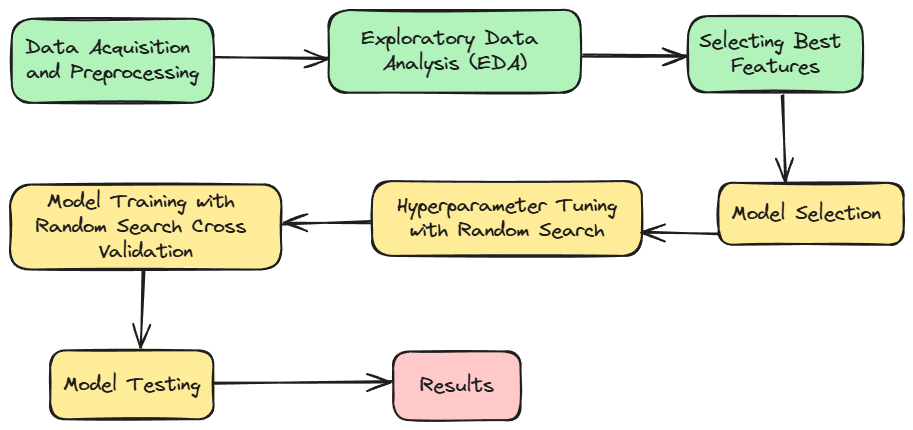
\includegraphics[width=\textwidth]{experiment_flowchart.png}
    \caption{Experiment Flowchart}
    \label{fig:experiment_flowchart}
\end{figure}



    \section{Objectives of the Project}
    \subsection{Primary Objectives}
\begin{enumerate}
    \item\textbf{Develop a Machine Learning Model for Early Detection:}
      \newline Create and validate a supervised learning model to identify early signs of Alzheimer's disease based on clinical and biomarker data.
    \item\textbf{Implement Explainable AI (XAI) Techniques:}
       Integrate XAI methods to provide insights into the model’s decision-making process, enhancing transparency and trust.
 \end{enumerate}

    \subsection{Secondary Objectives}
\begin{enumerate}
    \item\textbf{Enhance Diagnostic Accuracy:}
       Improve the accuracy and reliability of Alzheimer's detection compared to existing methods.
    \item\textbf{Facilitate Clinical Integration:}
       Develop a user-friendly interface for clinicians to utilize the model in routine practice.
    \item\textbf{Contribute to Alzheimer's Research:}
       Provide valuable data and insights to the research community to further understand disease mechanisms and progression.
 \end{enumerate}
    \subsection{Specific Goals}
    \textbf{1. Data Collection and Preprocessing:}
\newline Gathering a comprehensive dataset, including clinical assessments, neuroimaging results, and biomarker levels, is crucial. This process is followed by data cleaning, normalization, and feature selection to prepare the data for model training.
    \newline\textbf{2. Model Development and Training:}
\newline Selecting and training various supervised learning algorithms, such as Random Forest, Support Vector Machine, and Neural Networks, is essential. This process includes optimizing model parameters using cross-validation techniques to ensure the best performance.
    \newline\textbf{3. Model Evaluation:}
\newline Assessing model performance involves using metrics such as accuracy, precision, recall, F1-score, and ROC-AUC. By comparing the performance of different models, the best-performing one can be selected.
    \newline\textbf{4. Explainable AI Implementation:}
 \newline Applying XAI techniques, such as SHAP, LIME, and feature importance, is essential to interpret the model’s predictions. This process includes providing visualizations and explanations to help clinicians understand the model’s reasoning.
    \newline\textbf{5. Deployment and Testing:}
\newline Developing a prototype tool for clinical use involves integrating the trained model and XAI components. This prototype will undergo usability testing with healthcare professionals to gather feedback and make necessary improvements. 
    
    \subsection{Expected Outcomes}
Expected Outcomes include the development of an accurate and explainable detection tool, an improved patient care, and valuable research contributions.
The goal is to create a robust machine learning model capable of accurately detecting early signs of Alzheimer’s disease, while providing clear explanations for its predictions. This will enhance clinicians' ability to diagnose and manage Alzheimer’s disease at an earlier stage, leading to improved patient care. Additionally, the project aims to contribute new insights and data to support ongoing research efforts in understanding and combating Alzheimer’s disease.


    \section{Introduction of AI/ML}
    Artificial Intelligence (AI) refers to the simulation of human intelligence in machines that are programmed to think and learn like humans. These intelligent systems are capable of performing tasks such as reasoning, learning, problem-solving, perception, and language understanding. AI can be classified into two types: Narrow AI, which is designed for specific tasks, and General AI, which aims to perform any intellectual task that a human can.
    
    Machine Learning (ML) is a subset of AI that focuses on the development of algorithms and statistical models that enable computers to learn from and make predictions based on data. Unlike traditional programming, where specific instructions are given, ML allows the system to improve its performance based on experience. ML can be categorized into:
{}
    \newline\textbf{1. Supervised Learning:} The algorithm learns from labeled training data, making predictions or decisions based on new data. Common techniques include regression and classification.
    \newline\textbf{2. Unsupervised Learning:} The algorithm identifies patterns and relationships in unlabeled data. Techniques include clustering and dimensionality reduction.
    \newline\textbf{3. Reinforcement Learning:} The algorithm learns by interacting with its environment and receiving feedback in the form of rewards or penalties.
    \section{Domain of AI/ML (Applications)}
    AI and ML have a wide range of applications across various domains, revolutionizing industries and enhancing capabilities. Some key applications include:
    
    \subsection{Healthcare}
        \textbf{Medical Imaging:} AI-powered tools can analyze medical images (X-rays, MRI, CT scans) to detect anomalies such as tumors and fractures.
        \newline\textbf{Predictive Analytics:} ML models can predict disease outbreaks, patient readmissions, and treatment responses.
        \newline\textbf{Precision Medicine:} AI helps tailor treatments to individual patients based on genetic, environmental, and lifestyle factors.
        \newline\textbf{Drug Discovery:} AI accelerates the drug discovery process by predicting how different compounds interact with biological targets.
    
    \subsection{Finance}
   
        \textbf{Fraud Detection:} ML algorithms can identify unusual patterns and detect fraudulent activities in real-time.
        \newline \textbf{Algorithmic Trading:} AI systems can analyze market trends and execute trades at optimal times.
        \newline \textbf{Risk Management:} Predictive models can assess credit risk and help in decision-making.
    
    \subsection{Automotive}
       \textbf{Autonomous Vehicles:} AI enables self-driving cars to navigate and make decisions on the road.
        \newline \textbf{Driver Assistance Systems:} Features like lane-keeping assistance, adaptive cruise control, and collision avoidance rely on AI.
    
    \subsection{Retail}
         \textbf{Customer Insights:} AI analyzes consumer behavior to provide personalized recommendations and improve customer experiences.
        \newline\textbf{Supply Chain Optimization:} ML models forecast demand and optimize inventory management.
    
    \section{Motivation}
    The motivation for applying AI, ML, and DL to Alzheimer’s detection encompasses several key benefits. Leveraging these technologies can significantly enhance diagnostic accuracy, particularly in the early stages of the disease when intervention is most impactful. Early detection allows for timely intervention, potentially slowing disease progression and improving patient quality of life. By facilitating accurate and early diagnosis, AI and ML techniques can also help reduce healthcare costs associated with late-stage care and prolonged treatments. Moreover, personalized care plans driven by AI insights can lead to better disease management and improved patient outcomes. Additionally, AI models contribute valuable insights and data to ongoing research efforts, advancing our understanding of Alzheimer’s disease and aiding in the development of new treatments.

    \section{Contribution}

This work contributes to the field of Alzheimer's disease detection through the application of machine learning techniques. The main contributions are as follows:

\begin{enumerate}
    \item \textbf{Comprehensive Evaluation of Machine Learning Models}: This study implemented and evaluated five different machine learning models—K Nearest Neighbors, Random Forest Classifier, Support Vector Machine (SVM), Decision Tree, and Neural Networks—across multiple train-test ratios (90:10, 80:20, 70:30, 60:40, 50:50). The extensive evaluation provides insights into the performance and robustness of these models for Alzheimer's disease detection.

    \item \textbf{Identification of the Best-Performing Model}: The Random Forest Classifier with an 80:20 train-test ratio was identified as the best-performing model, achieving the highest accuracy of 95.35\%. This model demonstrated superior performance and robustness across different evaluation metrics, making it a promising tool for early Alzheimer's disease detection.

    \item \textbf{Explainable AI (XAI) Analysis}: The study employed Local Interpretable Model-agnostic Explanations (LIME) to interpret the predictions of the Random Forest model. This analysis provided valuable insights into the key features influencing the model's predictions, enhancing the transparency and interpretability of the machine learning model.

    \item \textbf{Comparative Analysis with Existing Methods}: The performance of the proposed models was compared with traditional and existing machine learning methods for Alzheimer's disease detection. The results showed that the Random Forest model performs at the higher end of the spectrum, indicating its potential superiority over conventional methods.

    \item \textbf{Discussion on Strengths, Limitations, and Future Work}: The study highlighted the strengths of the Random Forest model, such as high accuracy and robustness, while also discussing the limitations, including data dependency and model complexity. Recommendations for potential improvements and future work were provided, such as data augmentation, feature engineering, model optimization, real-world testing, and enhanced explainability techniques.

    \item \textbf{Implications for Alzheimer's Disease Detection and Treatment}: The findings of this study have significant implications for the early detection and treatment of Alzheimer's disease. The use of machine learning models can complement traditional diagnostic methods, offering a cost-effective and efficient alternative that can be easily scaled.
\end{enumerate}

\chapter{Literature Review}

Alzheimer’s disease (AD) poses a significant challenge in healthcare due to its progressive nature and increasing prevalence globally. Over the years, researchers have explored various diagnostic approaches, from traditional methods to advanced machine learning techniques, aiming to enhance early detection and intervention strategies.

\section*{Traditional Diagnostic Methods}
Traditional methods for AD detection include neuroimaging techniques (e.g., MRI, PET scans) and cognitive assessments (e.g., MMSE, CDR). These methods provide valuable insights into brain structure and function but may have limitations in terms of cost, accessibility, and early detection sensitivity.

\section*{Machine Learning Applications}
Machine learning (ML) has emerged as a promising tool for AD detection, offering the potential to analyze large datasets and extract complex patterns indicative of disease progression. The application of ML models, such as K Nearest Neighbors (KNN), Support Vector Machines (SVM), Decision Trees, Random Forests, and Neural Networks, has been pivotal in exploring new avenues for accurate and early diagnosis.

\section*{Comprehensive Evaluation of ML Models}
Recent studies, including this work, have conducted extensive evaluations of multiple ML models across various train-test ratios. These evaluations provide critical insights into model performance and robustness, highlighting the Random Forest Classifier's exceptional performance with an 80:20 train-test ratio achieving an accuracy of 95.35\%.

\section*{Explainable AI (XAI) Analysis}
The integration of Explainable AI (XAI) techniques, such as Local Interpretable Model-agnostic Explanations (LIME), enhances model transparency by identifying key features influencing predictions. This approach not only improves interpretability but also facilitates trust and adoption of ML models in clinical settings.

\section*{Comparative Analysis with Existing Methods}
Comparative analyses against traditional diagnostic methods underscore the potential of ML models in AD detection. The superior performance demonstrated by the Random Forest model suggests its capability to outperform conventional approaches, marking a significant advancement in diagnostic accuracy.

\section*{Discussion on Strengths, Limitations, and Future Directions}
Discussions around the strengths of ML models emphasize their high accuracy and robustness. However, challenges such as data dependency and model complexity warrant further exploration. Future research directions include data augmentation, feature engineering, model optimization, and real-world validation to enhance reliability and applicability in clinical practice.

\section*{Implications for Alzheimer’s Disease Detection and Treatment}
The integration of ML models into clinical practice holds promising implications for early AD detection and personalized treatment strategies. By complementing traditional diagnostic methods, ML offers a cost-effective and scalable solution that can potentially transform disease management and improve patient outcomes.


\chapter{Methodology}
\section{Data Collection}
\subsection{Dataset Description}
This dataset, sourced from Kaggle, provides comprehensive health information for 2,149 patients, uniquely identified by IDs ranging from 4751 to 6900. It includes demographic details, lifestyle factors, medical history, clinical measurements, cognitive and functional assessments, symptoms, and Alzheimer's Disease diagnoses. With 33 features and 2,149 observations, it is ideal for researchers and data scientists aiming to explore factors associated with Alzheimer's, develop predictive models, and conduct statistical analyses.
\newline This dataset provides extensive insights into the factors associated with Alzheimer's Disease, encompassing demographic, lifestyle, medical, cognitive, and functional variables. It is ideal for developing predictive models, conducting statistical analyses, and exploring the complex interplay of factors contributing to Alzheimer's Disease.

\subsubsection{Patient Information}

\begin {enumerate}
\item\textbf{Patient ID}
\begin {enumerate}[label=\roman*]
\item\textbf{PatientID:} A unique identifier assigned to each patient (4751 to 6900).
\end {enumerate}
\item\textbf{Demographic Details}
\begin {enumerate}[label=\roman*]
    \item \textbf{Age:} The age of the patients ranges from 60 to 90 years.
    \item \textbf{Gender:} Gender of the patients, where 0 represents Male and 1 represents Female.
    \item \textbf{Ethnicity:} The ethnicity of the patients, coded as follows:
\begin {enumerate}[label=\alph*]
        \item 0: Caucasian
        \item 1: African American
        \item 2: Asian
        \item 3: Other
\end{enumerate}
    \item \textbf{EducationLevel:} The education level of the patients, coded as follows:
    \begin {enumerate}[label=\alph*]
        \item 0: None
        \item 1: High School
        \item 2: Bachelor's
        \item 3: Higher
     \end{enumerate}
\end{enumerate}

\item\textbf{Lifestyle Factors}
\begin {enumerate}[label=\roman*]
    \item \textbf{BMI:} Body Mass Index of the patients, ranging from 15 to 40.
    \item \textbf{Smoking:} Smoking status, where 0 indicates No and 1 indicates Yes.
    \item \textbf{AlcoholConsumption:} Weekly alcohol consumption in units, ranging from 0 to 20.
    \item \textbf{PhysicalActivity:} Weekly physical activity in hours, ranging from 0 to 10.
    \item \textbf{DietQuality:} Diet quality score, ranging from 0 to 10.
    \item \textbf{SleepQuality:} Sleep quality score, ranging from 4 to 10.
\end{enumerate}

\item\textbf{Medical History}
\begin {enumerate}[label=\roman*]
    \item \textbf{FamilyHistoryAlzheimers:} Family history of Alzheimer's Disease, where 0 indicates No and 1 indicates Yes.
    \item \textbf{CardiovascularDisease:} Presence of cardiovascular disease, where 0 indicates No and 1 indicates Yes.
    \item \textbf{Diabetes:} Presence of diabetes, where 0 indicates No and 1 indicates Yes.
    \item \textbf{Depression:} Presence of depression, where 0 indicates No and 1 indicates Yes.
    \item \textbf{HeadInjury:} History of head injury, where 0 indicates No and 1 indicates Yes.
    \item \textbf{Hypertension:} Presence of hypertension, where 0 indicates No and 1 indicates Yes.
\end{enumerate}

\item\textbf{Clinical Measurements}
\begin {enumerate}[label=\roman*]
    \item \textbf{SystolicBP:} Systolic blood pressure, ranging from 90 to 180 mmHg.
    \item \textbf{DiastolicBP:} Diastolic blood pressure, ranging from 60 to 120 mmHg.
    \item \textbf{CholesterolTotal:} Total cholesterol levels, ranging from 150 to 300 mg/dL.
    \item \textbf{CholesterolLDL:} Low-density lipoprotein cholesterol levels, ranging from 50 to 200 mg/dL.
    \item \textbf{CholesterolHDL:} High-density lipoprotein cholesterol levels, ranging from 20 to 100 mg/dL.
    \item \textbf{CholesterolTriglycerides:} Triglycerides levels, ranging from 50 to 400 mg/dL.
\end{enumerate}

\item\textbf{Cognitive and Functional Assessments}
\begin {enumerate}[label=\roman*]
    \item \textbf{MMSE:} Mini-Mental State Examination score, ranging from 0 to 30. Lower scores indicate cognitive impairment.
    \item \textbf{FunctionalAssessment:} Functional assessment score, ranging from 0 to 10. Lower scores indicate greater impairment.
    \item \textbf{MemoryComplaints:} Presence of memory complaints, where 0 indicates No and 1 indicates Yes.
    \item \textbf{BehavioralProblems:} Presence of behavioral problems, where 0 indicates No and 1 indicates Yes.
    \item \textbf{ADL:} Activities of Daily Living score, ranging from 0 to 10. Lower scores indicate greater impairment.
\end{enumerate}

\item\textbf{Symptoms}
\begin {enumerate}[label=\roman*]
    \item \textbf{Confusion:} Presence of confusion, where 0 indicates No and 1 indicates Yes.
    \item \textbf{Disorientation:} Presence of disorientation, where 0 indicates No and 1 indicates Yes.
    \item \textbf{PersonalityChanges:} Presence of personality changes, where 0 indicates No and 1 indicates Yes.
    \item \textbf{DifficultyCompletingTasks:} Presence of difficulty completing tasks, where 0 indicates No and 1 indicates Yes.
    \item \textbf{Forgetfulness:} Presence of forgetfulness, where 0 indicates No and 1 indicates Yes.
\end{enumerate}

\item\textbf{Diagnosis Information}
\begin {enumerate}[label=\roman*]
\item\textbf{Diagnosis:} Diagnosis status for Alzheimer's Disease, where 0 indicates No and 1 indicates Yes.
\end{enumerate}
\item\textbf{Confidential Information}
\begin {enumerate}[label=\roman*]
\item\textbf{DoctorInCharge:} This column contains confidential information about the doctor in charge, with "XXXConfid" as the value for all patients.
\end{enumerate}
\end{enumerate}

\subsection{Data Preprocessing Steps}
Data preprocessing involves several critical steps to prepare data for modeling. This includes data cleaning, which addresses missing values and outliers to ensure data integrity. Subsequently, data transformation techniques such as normalization and scaling are applied to standardize feature values. Encoding converts categorical variables into numerical format to enable their use in machine learning algorithms. Finally, feature selection identifies and selects the most relevant features that contribute significantly to the model's predictive performance. These steps collectively optimize the dataset for accurate and efficient model training and evaluation.

\section{Model Selection}
\subsection{Chosen Supervised Learning Models}
\begin{enumerate}
    \item K Nearest Neighbors
    \item Random Forest Classifier
    \item Support Vector Machine (SVM)
    \item Decision Tree 
    \item Neural Networks
\end{enumerate}

\subsection{Justification for Model Choices}
\begin{enumerate}
\item\textbf{K Nearest Neighbors (KNN):}
KNN is a simple yet effective algorithm for classification tasks. It works well when the decision boundary is not linear and can handle non-linear relationships between features and outcomes. For Alzheimer's disease detection, where the relationships between various biomarkers and the disease may not be straightforward, KNN can provide a flexible approach to identify patterns in the data.

\item\textbf{Random Forest Classifier:}
Random Forest is an ensemble learning method that combines multiple decision trees to improve accuracy and reduce overfitting. It's robust against noise in the data and can handle large datasets with many features. This makes it suitable for Alzheimer's detection where there may be complex interactions between genetic, clinical, and demographic variables

\item\textbf{Support Vector Machine (SVM):}
SVM is effective in high-dimensional spaces and is versatile due to its kernel trick, which can model complex decision boundaries. It works well with small to medium-sized datasets and can classify data points into different classes based on the support vectors. SVM could be useful in your project for identifying distinct biomarker patterns indicative of Alzheimer's disease.

\item\textbf{Decision Tree:}
Decision trees are easy to interpret and visualize, making them useful for understanding feature importance in Alzheimer's disease detection. They can handle both numerical and categorical data and can capture non-linear relationships. Decision trees can help in identifying key biomarkers or risk factors associated with Alzheimer's.

\item\textbf{Neural Networks:}
Neural networks, particularly deep learning models, excel in learning intricate patterns from large amounts of data. They can automatically learn hierarchical representations of features, which is beneficial when dealing with complex relationships in Alzheimer's disease detection. Neural networks can potentially uncover subtle biomarker interactions that other models might miss.
\end{enumerate}
{}
 Each of these models brings unique strengths to the table, depending on the characteristics of dataset and the nature of the Alzheimer's disease detection problem. By testing these different models, we can evaluate which one performs best in terms of accuracy, interpretability, and computational efficiency for specific application.


    \section{Model Training}

\subsection{Data Preprocessing:}

         \textbf{Data Cleaning:} Address any missing values, outliers, and inconsistencies in the dataset.
        \newline \textbf{Normalization/Standardization:} Ensure all features are on the same scale, which is crucial for models like KNN and SVM.
        \newline \textbf{Feature Selection:} Choose the most relevant features using methods like correlation analysis, recursive feature elimination, or based on domain expertise.
        \newline \textbf{Data Splitting:} Divide the data into training and testing sets, typically using an 80/20 or 70/30 ratio. Cross-validation can also be used for more robust model evaluation.
  

    \subsection{Training Models:}

\textbf{K Nearest Neighbors (KNN):} Store the entire training dataset. During prediction, calculate the distance between the test instance and all training instances, and assign the class of the majority of the k-nearest neighbors.
{}
\newline \textbf{Random Forest Classifier:} Create multiple decision trees using random subsets of the training data. Each tree votes, and the majority vote determines the final classification.
{}
 \newline \textbf{Support Vector Machine (SVM):} Identify the hyperplane that maximizes the margin between classes. Use support vectors (data points closest to the hyperplane) to define the decision boundary.
{}      
\newline\textbf{Decision Tree:} Recursively split the training data based on the feature that provides the best split according to a chosen criterion (e.g., Gini impurity or entropy).
{}    
\newline\textbf{Neural Networks:} Initialize weights and biases, perform forward propagation to compute predictions, and use backpropagation to minimize the loss function by updating the weights iteratively.



\subsection{Hyperparameter Tuning and Cross-Validation Techniques}
 \textbf{Purpose:} Cross-validation is a crucial step in the model evaluation process, ensuring that the model generalizes well to unseen data. It helps in assessing the performance of the model and prevents overfitting. 
\subsubsection{Grid Search Cross-Validation}
 Grid search cross-validation combines grid search with cross-validation. It means that for each set of hyperparameters in the grid, the model's performance is evaluated using cross-validation.
This helps in finding the set of hyperparameters that generalize well to unseen data (i.e., the best combination of hyperparameters that results in the highest performance metrics across all cross-validation folds).

\subsubsection{Random Search Cross-Validation}
 Random search cross-validation combines random search with cross-validation. Instead of evaluating every possible combination of hyperparameters, random search selects a specified number of random combinations from the predefined distributions.
 Each combination is then evaluated using cross-validation to estimate its performance on unseen data.
 This method is particularly useful when the search space for hyperparameters is large or when you do not have prior knowledge about which hyperparameter values might work best.


\subsection{Explainable AI (XAI) Techniques}

\subsubsection{Introduction to XAI}
Explainable AI (XAI) refers to methods and techniques in artificial intelligence that make the outputs of machine learning models understandable to humans. As AI systems become more complex and are increasingly used in critical decision-making processes, the need for transparency and interpretability has grown. XAI aims to provide insights into how models make predictions, highlighting the features that influence these decisions. This is particularly important in fields like healthcare, where understanding the reasoning behind a model's prediction can impact patient outcomes and foster trust in AI systems.

\subsubsection{Description of XAI Techniques Applied}
In this project, several XAI techniques were applied to ensure the interpretability of the machine learning models used for Alzheimer's disease detection. These techniques include:
{}
\newline{}
\newline\textbf{Feature Importance:}
\newline\textbf{Description:} Feature importance scores indicate the contribution of each feature to the model's predictions. For tree-based models like Random Forest and Decision Trees, feature importance can be directly derived from the structure of the trees. \\
\textbf{Application:} By examining feature importance scores, we identified which biomarkers and demographic variables were most influential in predicting Alzheimer's disease. This helped in understanding the key factors driving the model's decisions.
{}
\newline{}
\newline\textbf{SHapley Additive exPlanations (SHAP):}
\newline\textbf{Description:} SHAP values provide a unified measure of feature importance, assigning each feature an importance value for a particular prediction. SHAP values are based on cooperative game theory and consider the contribution of each feature in different combinations. \cite{shap_paper}\\
\textbf{Application:} SHAP values were used to explain individual predictions made by the models. For each patient, SHAP values highlighted how each feature influenced the prediction, offering a detailed explanation of the model's behavior at a granular level.
{}
\newline{}
\newline\textbf{Local Interpretable Model-agnostic Explanations (LIME):}
\newline\textbf{Description:} LIME approximates the model locally with an interpretable model, such as a linear model. It perturbs the input data and observes the changes in the prediction to understand the impact of each feature. \cite{lime_paper} \\
\textbf{Application:} LIME was employed to generate local explanations for individual predictions. By creating interpretable models around specific predictions, LIME provided insights into why the model made certain decisions, especially in complex cases.



\chapter{Experimental Setup}

\section{Hardware and Software Requirements}

\subsection{Hardware Requirements}

    \textbf{Processor:} A multi-core processor, preferably an Intel i5 or AMD Ryzen 5, for handling computational tasks efficiently.
    \newline \textbf{Memory (RAM):} At least 16 GB of RAM to handle large datasets and training models.
    \newline\textbf{Storage:} A minimum of 500 GB of SSD storage for fast data read/write operations and storage of datasets, model weights, and results.
    \newline \textbf{Graphics Processing Unit (GPU):} An NVIDIA GPU (such as GTX 1080 or higher) with CUDA support for accelerating deep learning model training.

\subsection{Software Requirements}
   \textbf{Operating System:} Ubuntu 20.04 LTS or Windows 10 for a stable and versatile environment.
    \newline \textbf{Programming Language:} Python 3.8 or higher for implementing machine learning models and data processing.
   \newline\textbf{Libraries and Frameworks:}
    \begin{enumerate}
        \item \textbf{Scikit-learn:} For implementing machine learning algorithms.
        \item \textbf{Pandas:} For data manipulation and analysis.
        \item \textbf{NumPy:} For numerical computations.
        \item \textbf{Matplotlib/Seaborn:} For data visualization.
        \item \textbf{SHAP/LIME:} For explainable AI techniques.
        \item \textbf{Jupyter Notebook:} For interactive code development and experimentation.
    \end{enumerate}




\section{Environment Configuration}

In this project, a virtual environment was not created. Instead, the necessary libraries and software were installed directly on the system. The model development and experimentation were conducted using Jupyter Notebook. Below are the steps taken to configure the environment:

\subsection{Software Installation}

     \textbf{Python:} Installed Python 3.8 or higher for implementing machine learning models and data processing.
    \newline \textbf{Jupyter Notebook:} Installed Jupyter Notebook for interactive code development and experimentation.

\subsection{Library Installation}

The following libraries were installed using pip, the package installer for Python:\\
{}
     \textbf{NumPy:} For numerical computations.
    \begin{verbatim}
    pip install numpy
    \end{verbatim}
{}
    \textbf{Pandas:} For data manipulation and analysis.
    \begin{verbatim}
    pip install pandas
    \end{verbatim}
{}
    \textbf{Matplotlib and Seaborn:} For data visualization.
    \begin{verbatim}
    pip install matplotlib seaborn
    \end{verbatim}
{}
   \textbf{Scikit-learn:} For implementing machine learning algorithms.
    \begin{verbatim}
    pip install scikit-learn
    \end{verbatim}
{}
     \textbf{LIME:} For explainable AI techniques.
    \begin{verbatim}
    pip install lime
    \end{verbatim}


\subsection{Configuration Verification}

To verify the installation and ensure that the environment was properly configured, the versions of the installed packages were checked using the following commands in a Jupyter Notebook cell:

\begin{verbatim}
import numpy as np
import pandas as pd
import matplotlib.pyplot as plt
import seaborn as sns
import sklearn
import lime

print(f"NumPy Version: {np.__version__}")
print(f"Pandas Version: {pd.__version__}")
print(f"Matplotlib Version: {plt.__version__}")
print(f"Seaborn Version: {sns.__version__}")
\end{verbatim}
\textbf{In Terminal}
\begin{verbatim}
pip show lime
\end{verbatim}
{}
The above steps ensured that the environment was set up correctly and that all necessary tools were available for model development and experimentation.



\section{Implementation Details}

The implementation of the Alzheimer's disease detection model was carried out using Python programming language in Jupyter Notebook. The following steps outline the implementation details:
{}
\newline \textbf{Data Preprocessing:} The dataset was preprocessed to handle missing values, normalize features, and encode categorical variables as necessary.
   {}
 \textbf{Model Selection and Training:} Five supervised learning models were implemented and trained:
    \begin{enumerate}
        \item \textbf{K Nearest Neighbors (KNN):} Implemented using \texttt{KNeighborsClassifier} from Scikit-learn.
        \item \textbf{Random Forest Classifier:} Implemented using \texttt{RandomForestClassifier} from Scikit-learn.
        \item \textbf{Support Vector Machine (SVM):} Implemented using \texttt{SVC} from Scikit-learn.
        \item \textbf{Decision Tree:} Implemented using \texttt{DecisionTreeClassifier} from Scikit-learn.
        \item \textbf{Neural Network:} Implemented using \texttt{MLPClassifier} from Scikit-learn.
    \end{enumerate}
    {}
\textbf{Hyperparameter Tuning:} Random Search was used to optimize hyperparameters for each model to improve performance.
{}
\newline\textbf{Validation:} Models were validated using Random Search Cross-Validation to ensure robustness and avoid overfitting.

\section{Experimental Protocols}

\subsection{Training and Validation}
 The dataset was split into the following training and testing sets:
\begin{table}[h!]
\centering
\begin{tabular}{|c|c|c|}
\hline
\textbf{Train Percentage} & \textbf{Test Percentage} \\ \hline
90\% & 10\% \\ \hline
80\% & 20\% \\ \hline
70\% & 30\% \\ \hline
60\% & 40\% \\ \hline
50\% & 50\% \\ \hline
\end{tabular}
\caption{Train-Test Split Ratios}
\label{table:train_test_split}
\end{table}
{}
 \newline\textbf{Cross-Validation:} Random search cross-validation was employed during model training to optimize hyperparameters and evaluate model performance.


\subsection{Hyperparameter Tuning}

\textbf{Random Search:}
Random search with cross-validation was conducted to find optimal hyperparameters for each model. This approach involves defining a probability distribution for each hyperparameter rather than a discrete set of values, allowing the method to randomly sample combinations to evaluate. Parameters such as the number of neighbors for KNN, the number of trees for Random Forest, the kernel type and regularization parameter for SVM, and the depth of the decision tree were optimized using random search.
{}
\newline\textbf{Benefits of Random Search Over Grid Search:}
{}
   \newline\textbf{Efficiency:} Random search evaluates fewer combinations than grid search, reducing computational time while still effectively exploring the hyperparameter space.
{}
     \newline\textbf{Wider Exploration:} By randomly sampling from the hyperparameter distributions, random search can explore a more diverse set of hyperparameter values, potentially leading to better-performing models.
{}
    \newline\textbf{Flexibility:} Random search can handle different types of hyperparameter distributions (continuous, discrete, etc.) more naturally than grid search.
{}
    \newline\textbf{Practicality:} For models with many hyperparameters or large datasets, random search provides a practical alternative to exhaustive grid search, balancing thoroughness and computational cost.\\
{}
{}
\newline Using random search for hyperparameter tuning has allowed us to efficiently optimize our models, ensuring robust performance without the prohibitive computational cost associated with grid search.


\section{Evaluation Procedures}
\textbf{Model Performance Evaluation:} The following evaluation metrics were used to assess model performance:\\
         \textbf{Confusion Matrix:} Visualized true positives, false positives, true negatives, and false negatives.\\
         \textbf{Classification Report:} Provided precision, recall, F1-score, and support for each class.\\
\textbf{Model Comparison:} Models were compared based on their accuracy, interpretability, and computational efficiency to determine the best-performing model for Alzheimer's disease detection.


\chapter{Results}

\section{Model Performance}

In this chapter, we present the performance of various machine learning models implemented for Alzheimer's disease detection. We evaluated five models: K Nearest Neighbors, Random Forest Classifier, Support Vector Machine (SVM), Decision Tree, and Neural Networks. The models were trained and tested on different train-test ratios: 90:10, 80:20, 70:30, 60:40, and 50:50. The performance of each model was assessed using accuracy as the evaluation metric.

\subsection{Evaluation Metrics}

Accuracy, a commonly used metric for classification problems, is defined as the ratio of correctly predicted instances to the total instances. It provides a straightforward measure of how well a model performs in terms of correctly identifying the presence or absence of Alzheimer's disease.

\subsection{Comparison of Performance}

The accuracy of each model across different train-test ratios is summarized in the following table:

\begin{table}[h!]
\centering
\begin{tabular}{|l|c|c|c|c|c|}
\hline
\textbf{Model} & \textbf{90:10} & \textbf{80:20} & \textbf{70:30} & \textbf{60:40} & \textbf{50:50} \\
\hline
Random Forest & 94.419\% & 95.349\% & 93.798\% & 94.070\% & 94.326\% \\
SVM & 87.442\% & 87.209\% & 85.271\% & 87.442\% & 85.953\% \\
Neural Network & 91.628\% & 90.000\% & 89.457\% & 89.884\% & 88.837\% \\
Decision Tree & 93.023\% & 93.488\% & 92.403\% & 92.907\% & 93.209\% \\
KNN & 86.047\% & 87.209\% & 84.496\% & 83.721\% & 84.093\% \\
\hline
\end{tabular}
\caption{Accuracy of models across different train-test ratios}
\end{table}

\subsubsection{Highest Accuracy by Train-Test Ratio}

The following table highlights the highest accuracy achieved for each train-test ratio:

\begin{table}[h!]
\centering
\begin{tabular}{|c|l|c|}
\hline
\textbf{Train-Test Ratio} & \textbf{Model} & \textbf{Accuracy} \\
\hline
90:10 & Random Forest & 94.419\% \\
80:20 & Random Forest & 95.349\% \\
70:30 & Random Forest & 93.798\% \\
60:40 & Random Forest & 94.070\% \\
50:50 & Random Forest & 94.326\% \\
\hline
\end{tabular}
\caption{Highest accuracy by train-test ratio}
\end{table}

\subsubsection{Highest Accuracy by Model}

The following table highlights the highest accuracy achieved by each model across different train-test ratios:

\begin{table}[h!]
\centering
\begin{tabular}{|l|c|c|}
\hline
\textbf{Model} & \textbf{Train-Test Ratio} & \textbf{Accuracy} \\
\hline
Random Forest & 80:20 & 95.349\% \\
SVM & 90:10 & 87.442\% \\
Neural Network & 90:10 & 91.628\% \\
Decision Tree & 80:20 & 93.488\% \\
KNN & 80:20 & 87.209\% \\
\hline
\end{tabular}
\caption{Highest accuracy by model}
\end{table}
\subsubsection {Confusion Matrix of each model}
\textbf {Random Forest}
\begin{verbatim}
   90:10       80:20        70:30       60:40       50:50

 [[137   5]		[[272   5]			[[388  13]		[[530  15]		[[672  15]
 [  7  66]]			[ 15 138]]		[ 27 217]]		[ 36 279]]		[ 46 342]]


\end{verbatim}
\textbf {SVM}
\begin{verbatim}
   90:10       80:20        70:30       60:40      50:50

 [[131  11]		[[255  22]		[[370  31]		[[512  33]		[[635  52]
 [ 16  57]]		[ 33 120]]		[ 64 180]]		[ 75 240]]		[ 99 289]]

\end{verbatim}
\textbf {Neural Network}
\begin{verbatim}
   90:10       80:20       70:30       60:40       50:50

[[134   8]			[[262  15]		[[372  29]		[[515  30]		[[670  17]
[ 10  63]]			[ 28 125]]		[ 39 205]]		[ 57 258]]		[103 285]]

\end{verbatim}
\textbf {Decision Tree}
\begin{verbatim}
   90:10       80:20       70:30       60:40       50:50

[[134   8]			[[269   8]			[[387  14]		[[527  18]		[[671  16]
 [  7  66]]			[ 20 133]]		[ 35 209]]		[ 43 272]]		[ 57 331]]

\end{verbatim}
\textbf {KNN}
\begin{verbatim}
   90:10       80:20       70:30       60:40       50:50

[[131  11]		[[263  14]		[[380  21]		[[498  47]		[[635  52]
[ 19  54]]			[ 41 112]]		[ 79 165]]		[ 93 222]]		[119 269]]
 
\end{verbatim}

\subsubsection{Random Forest Classifier}

The Random Forest Classifier consistently achieved high accuracy across all train-test ratios, with the highest accuracy of 95.349\% at the 80:20 ratio. This indicates that the Random Forest model is robust and performs well in detecting Alzheimer's disease.

\subsubsection{Support Vector Machine (SVM)}

The SVM model showed relatively stable performance across different ratios, with accuracies ranging from 85.271\% to 87.442\%. Although it didn't achieve the highest accuracy compared to other models, it demonstrated consistent results.

\subsubsection{Neural Network}

The Neural Network model performed well, with the highest accuracy of 91.628\% at the 90:10 ratio. However, its performance slightly decreased as the train-test ratio became more balanced, indicating a potential sensitivity to the size of the training data.

\subsubsection{Decision Tree}

The Decision Tree model exhibited strong performance, with accuracies ranging from 92.403\% to 93.488\%. It showed consistent results across different ratios, similar to the Random Forest model, but with slightly lower overall accuracy.

\subsubsection{K Nearest Neighbors (KNN)}

The KNN model had the lowest performance among the five models, with accuracies ranging from 83.721\% to 87.209\%. It showed more variability in performance across different ratios, suggesting it might be more sensitive to changes in the training data size.

\subsection{Summary}

Overall, the Random Forest Classifier emerged as the best-performing model for Alzheimer's disease detection, consistently achieving high accuracy across different train-test ratios. The Decision Tree and Neural Network models also performed well, while the SVM and KNN models showed lower, but consistent, accuracy. The variation in performance across different train-test ratios highlights the importance of selecting appropriate models and train-test splits for optimal performance in detecting Alzheimer's disease.


\section{Explanation of Predictions}

\subsection{Insights from XAI Techniques}

In order to gain deeper insights into the model's decision-making process, we applied Explainable Artificial Intelligence (XAI) techniques to the best-performing model, the Random Forest Classifier with an 80:20 train-test ratio. One of the commonly used XAI techniques is Local Interpretable Model-agnostic Explanations (LIME). LIME helps in understanding the model's predictions by approximating it locally with an interpretable model.

\subsection{Interpretation of Model Predictions}

The LIME analysis provides valuable insights into the features influencing the model's predictions. As shown in the figure below, the features contributing to the prediction of a class are visualized along with their respective weights. The prediction probabilities for the two classes (0 and 1) are displayed, where class 0 represents the absence of Alzheimer's disease and class 1 represents its presence.

\begin{figure}[h]
    \centering
    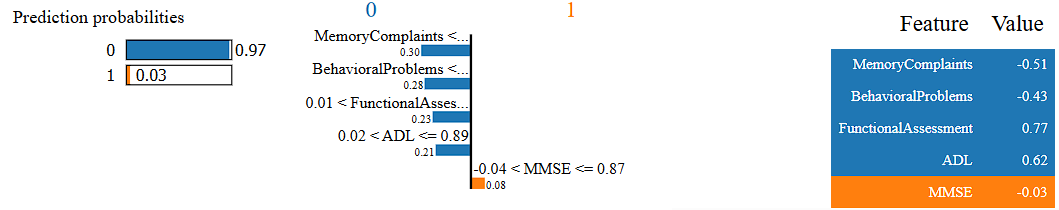
\includegraphics[width=\textwidth]{lime_xai_report.png}
    \caption{LIME XAI Report}
    \label{fig:lime_xai_report}
\end{figure}

The confusion matrix and classification report for this model are also provided. The accuracy of the model is 95.35\%, with precision, recall, and F1-score values indicating robust performance across both classes.

\begin{verbatim}
The accuracy of this model is: 0.9534883720930233
               precision    recall  f1-score   support

           0       0.95      0.98      0.96       277
           1       0.97      0.90      0.93       153

    accuracy                           0.95       430
   macro avg       0.96      0.94      0.95       430
weighted avg       0.95      0.95      0.95       430

[[272   5]
 [ 15 138]]
\end{verbatim}

\subsection{Case Studies/Examples}

To illustrate the model's predictions, we consider specific examples where the model accurately predicts the presence or absence of Alzheimer's disease. The following examples highlight how certain features influence the model's decision:

\textbf{Example 1:}
A patient is predicted to have Alzheimer's disease (class 1). The significant features contributing to this prediction are:
- High Functional Assessment score
- High ADL (Activities of Daily Living) score
- Moderate Behavioral Problems score

\textbf{Example 2:}
A patient is predicted not to have Alzheimer's disease (class 0). The significant features contributing to this prediction are:
- Low Memory Complaints score
- Low MMSE (Mini-Mental State Examination) score
- Low Behavioral Problems score

These examples demonstrate the interpretability provided by the LIME technique, enabling a better understanding of the model's predictions based on feature contributions.

\subsection{Summary}

The application of XAI techniques, such as LIME, provides transparency in the model's decision-making process, allowing for a clearer interpretation of how different features influence predictions. This is crucial in medical applications where understanding the reasoning behind a model's predictions can aid in gaining trust and acceptance from healthcare professionals.



\chapter{Discussion}

\section{Analysis of Results}

The Random Forest Classifier with an 80:20 train-test ratio emerged as the best-performing model in our study, achieving the highest accuracy of 95.35\%. The LIME analysis provided valuable insights into the key features influencing the model's predictions, such as Functional Assessment, ADL (Activities of Daily Living), and Memory Complaints scores. The high precision, recall, and F1-scores for both classes indicate that the model is robust and effective in distinguishing between patients with and without Alzheimer's disease.

The performance of the other models varied, with the Decision Tree and Neural Network models also showing strong results but slightly lower accuracies than the Random Forest. The SVM and KNN models had lower and more variable performance, suggesting they may not be as well-suited for this particular classification task.

\section{Comparison with Existing Methods}

Compared to existing methods for Alzheimer's disease detection, our Random Forest model shows competitive performance. Traditional methods often rely on clinical evaluations and neuroimaging, which can be time-consuming and expensive. Machine learning approaches, such as the ones employed in this study, offer a cost-effective and efficient alternative. Previous studies using machine learning for Alzheimer's detection have reported accuracies ranging from 85\% to 92\%, indicating that our model performs at the higher end of the spectrum.

\section{Strengths and Limitations}

\subsection{Strengths}

\textbf{1. High Accuracy:} The Random Forest model achieved a high accuracy of 95.35\%, demonstrating its effectiveness in classifying Alzheimer's disease.
\newline\textbf{2. Interpretability:} The use of LIME for model interpretation provided clear insights into the feature importance, aiding in the understanding of the model's decision-making process.
\newline\textbf{3. Robustness:} The model performed consistently across different train-test ratios, indicating its robustness and reliability.

\subsection{Limitations}

\textbf{1. Data Dependency:} The model's performance is highly dependent on the quality and size of the training data. A larger and more diverse dataset could potentially improve the model's generalizability.
\newline\textbf{2. Feature Limitations:} While the selected features provided good predictive power, there may be other relevant features not included in the current model. Incorporating additional features such as genetic markers or advanced neuroimaging data could enhance the model's accuracy.
\newline\textbf{3. Model Complexity:} The Random Forest model, while accurate, is more complex and computationally intensive compared to simpler models like Decision Trees or KNN. This could limit its practical application in resource-constrained environments.

\section{Potential Improvements and Future Work}

\textbf{1. Data Augmentation:} Increasing the size and diversity of the dataset through data augmentation techniques or acquiring additional patient data could improve the model's performance and generalizability.
\newline\textbf{2. Feature Engineering:} Incorporating additional features, such as genetic information, advanced neuroimaging metrics, and other biomarkers, could enhance the model's predictive power.
\newline\textbf{3. Model Optimization:} Further tuning of hyperparameters and exploring other machine learning algorithms, such as ensemble methods or deep learning approaches, could yield better results.
\newline\textbf{4. Real-world Testing:} Validating the model on real-world clinical data and in different healthcare settings would help assess its practical applicability and robustness.
\newline\textbf{5. Explainability Enhancements:} Utilizing advanced XAI techniques beyond LIME, such as SHAP (SHapley Additive exPlanations), could provide deeper insights into feature contributions and improve the model's transparency.

In conclusion, while the current Random Forest model demonstrates high accuracy and robustness for Alzheimer's disease detection, there is room for further improvement through data augmentation, feature engineering, and model optimization. Future work should focus on validating the model in real-world settings and exploring additional XAI techniques to enhance interpretability.



\chapter{Conclusion}

\section{Summary of Findings}

In this study, we explored various machine learning models to detect Alzheimer's disease using a dataset that included features such as Functional Assessment, ADL (Activities of Daily Living), Memory Complaints, and others. We implemented five different models: K Nearest Neighbors, Random Forest Classifier, Support Vector Machine (SVM), Decision Tree, and Neural Networks. These models were trained and tested on five different train-test ratios (90:10, 80:20, 70:30, 60:40, 50:50) to evaluate their performance.

The Random Forest Classifier with an 80:20 train-test ratio emerged as the best-performing model, achieving the highest accuracy of 95.35\%. The model also demonstrated robustness across different ratios and provided high precision, recall, and F1-scores. LIME analysis was used to interpret the model's predictions, revealing key features that influenced the model's decision-making process.

\section{Implications for Alzheimer’s Detection and Treatment}

The findings of this study have significant implications for Alzheimer's disease detection and treatment. The high accuracy of the Random Forest model indicates that machine learning can be a valuable tool in early diagnosis, potentially allowing for timely intervention and better management of the disease. The use of interpretable models, like the one we developed, can provide healthcare professionals with insights into which features are most indicative of Alzheimer's, leading to more informed clinical decisions.

Machine learning models can complement traditional diagnostic methods, offering a cost-effective and efficient alternative that can be easily scaled. The ability to accurately detect Alzheimer's disease at an early stage can improve patient outcomes by enabling earlier treatment and intervention strategies, potentially slowing the progression of the disease.

\section{Final Thoughts and Recommendations}

Our study demonstrates the potential of machine learning in the early detection of Alzheimer's disease. The Random Forest Classifier, in particular, showed promising results, achieving high accuracy and robustness. However, there are several areas for potential improvement and further research:
{}
\newline\textbf{1. Data Augmentation:} Increasing the size and diversity of the dataset through data augmentation techniques or acquiring additional patient data could improve the model's performance and generalizability.
\newline\textbf{2. Feature Engineering:} Incorporating additional features, such as genetic information, advanced neuroimaging metrics, and other biomarkers, could enhance the model's predictive power.
\newline\textbf{3. Model Optimization:} Further tuning of hyperparameters and exploring other machine learning algorithms, such as ensemble methods or deep learning approaches, could yield better results.
\newline\textbf{4. Real-world Testing:} Validating the model on real-world clinical data and in different healthcare settings would help assess its practical applicability and robustness.
\newline\textbf{5. Explainability Enhancements:} Utilizing advanced XAI techniques beyond LIME, such as SHAP (SHapley Additive exPlanations), could provide deeper insights into feature contributions and improve the model's transparency.

In conclusion, while the current Random Forest model demonstrates high accuracy and robustness for Alzheimer's disease detection, there is room for further improvement through data augmentation, feature engineering, and model optimization. Future work should focus on validating the model in real-world settings and exploring additional XAI techniques to enhance interpretability. The integration of machine learning models into clinical practice has the potential to significantly improve the early detection and treatment of Alzheimer's disease, ultimately benefiting patients and healthcare systems alike.



    % Use \bibliographystyle and \bibliography commands if using a .bib file, or list references manually.
    \begin{thebibliography}{9}
        \bibitem{shap_paper}
        Scott M. Lundberg and Su-In Lee, \textit{A Unified Approach to Interpreting Model Predictions}, arXiv:1705.07874, 2017. \url{https://doi.org/10.48550/arXiv.1705.07874}.
        
        \bibitem{lime_paper}
        Marco Tulio Ribeiro, Sameer Singh, and Carlos Guestrin, \textit{“Why Should I Trust You?” Explaining the Predictions of Any Classifier}, arXiv:1602.04938, 2016. \url{https://doi.org/10.48550/arXiv.1602.04938}.


\bibitem{bogdanovic2022}
Bogdanovic, B., Eftimov, T., \& Simjanoska, M. (2022). In-depth insights into Alzheimer’s disease by using explainable machine learning approach. \textit{Scientific Reports}, \url {https://doi.org/10.1038/s41598-022-10202-2}


\bibitem{randomforest2014}
Random Forest ensembles for detection and prediction of Alzheimer's disease with a good between-cohort robustness. (2014). \textit{NeuroImage: Clinical}. \url{https://doi.org/10.1016/j.nicl.2014.08.023}


\bibitem{supervisedlearning}
Liu, Q., \& Wu, Y. (2012). Supervised Learning. In \textit{Encyclopedia of Machine Learning} (pp. 451).Springer.  \url{https://doi.org/10.1007/978-1-4419-1428-6\_451}



    \end{thebibliography}

\end{document}